%\documentclass[prd,showpacs,onecolumn]{amsart}
\documentclass[prd,showpacs,twocolumn]{revtex4-1}
\usepackage{graphicx}% Include figure files
\usepackage{epstopdf}
\usepackage{dcolumn}% Align table columns on decimal point
\usepackage{bm}% bold math
\usepackage{amsmath}
%\nofiles
\begin{document}
\title{A classical model of a particle passing double slits}
\author{Peifeng Wang}
\email{peifeng\_w@yahoo.com}
\address{Guanghua Road 1\#, 34-1-3-5, Yanta District, Xi'an, Shaanxi, P. R. China 710075}
\address{Mijiaqiao 34-1-5, Xi'an, Shaanxi, P. R. China 710075}
\begin{abstract}
A classical model is presented that, due to electric field, when a particle is passing double slits, a self induced force can arise so that the particle is impacted by both slits simultaneously to form concentration varying patterns. While this model may not precisely account for the interference fringes, it raises a question on the origin of the diffraction patterns and imposes restrictions on wave-particle duality.
\end{abstract}
\maketitle
%249489

Unlike the general perception that double slit experiment can only be possibly explained within quantum mechanics (see \cite{Juffmann,Bach} and references therein), a classical model is presented to show that wave-particle duality is insufficient to account for the double slit experiment. In addition, a single particle can be impacted by both slits simultaneously, thus wave-particle duality may not even be necessary for double slit experiment.

Conceptually, a particle passing a surface can induce a field that exerts a force on itself to change its own trajectory. More specifically, a double slit is a surface S with certain portion (the slits) removed, when a charged particle q (or a molecule as an electric dipole) is passing next to the surface S, charge opposite to q is induced on the surface with density $\sigma$, which will generate a field E, thus exert a force F on the original charge q. Due to the slit(s) on the surface S, the field E of the induced charge can have a lateral component, which pulls the charge q towards some regions while pushes the charge q away from other regions. The outcome would be concentration varying patterns, somewhat like those in a diffraction.

In the following discussion, a surface S is placed at plane z=0. Three configurations of the surface S are examined, each having no slit, one slit and two slits respectively. With the slits aligned along x axis, non vanishing lateral component of the induced field in the direction of y axis is computed as an integral over the surface S so that multiple slits on S can simultaneously have impact on a single passing charge q. We then study the applicability of the model to show that the various scenarios in the model may impose restriction on wave-particle duality.

The electric field $\mathbf E$ due to charge density $\rho(\mathbf{x'})$ is\cite{Jackson}
\begin{eqnarray}
&&\mathbf{E(x)}=\frac{1}{4\pi\epsilon_0}\int\rho(\mathbf{x'})\frac{\mathbf{x-x'}}{|\mathbf{x-x'}|^3}d^3x'
\label{eqn:Coulomb}
\end{eqnarray}

For induced charge on the surface S, the charge density $\rho$ becomes surface charge density $\sigma$. If $\hat{\mathbf y}$ is the unit vector in the direction of positive y axis, the lateral component of the induced field is
\begin{eqnarray}
E_y&&=\mathbf E\cdot\hat{\mathbf y}\nonumber\\
&&=\frac{1}{4\pi\epsilon_0}\int_S \frac{\sigma(x',y')(y-y')dx'dy'}{((x-x')^2+(y-y')^2+(z-z')^2)^{3/2}}
\label{eqn:Ey}
\end{eqnarray}
For the purpose of this discussion, we are mainly interested in the impact of $E_y$ on the passing charge q, so $(x,y,z)$ specifies the location of the passing charge q, while $(x',y',z')$ with $z'=0$ is the coordinates of the induced charge on the surface S.

In the first configuration, the surface S locates at z=0 with no slit on it. Assuming the surface is conducting and infinite, the Dirichlet boundary condition is
\begin{eqnarray}
&&\Phi(x',y',z'=0)=0
\label{eqn:Dirichlet0}
\end{eqnarray}
where $\Phi$ is the scalar potential such that $\mathbf E=-\nabla \Phi$. When charge q is placed next to the surface at $(x=0,y,z)$, as show in fig. \ref{fig:image},
\begin{figure}
\center
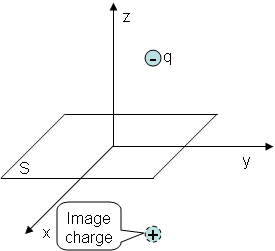
\includegraphics{noslit.png}
\caption{A conducting surface S is placed at plane z=0, a charge q at (0,y,z) and its image at (0,y,-z)}
\label{fig:image}
\end{figure}
the induced surface charge density can be obtained by method of image\cite{Jackson}
\begin{eqnarray}
&&\sigma(x',y')=\frac{-q}{2\pi\epsilon_0}\frac{|z|}{(x'^2+(y'-y)^2+z^2)^{3/2}}
\label{eqn:Sigma}
\end{eqnarray}
then the lateral component of induced field at charge q can be computed by substitution of (\ref{eqn:Sigma}) into (\ref{eqn:Ey}). Due to symmetry
\begin{eqnarray}
E_y(x=0,y,z)|_{0slit}=0
\label{eqn:Ey0}
\end{eqnarray}

In the second configuration, the surface S at z=0 has one slit along x axis, as shown in fig. \ref{fig:Single_Slit}a.
\begin{figure}
\center
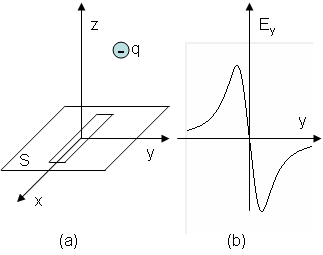
\includegraphics{1slit.png}
\caption{a) A conducting surface S is placed at plane z=0. On the surface, there is a slit along x axis with its center at the origin. A negative charge q is passing at (0,y,z). b) Sketch of the lateral component of the induced electric field at the location of the negative charge q}
\label{fig:Single_Slit}
\end{figure}
The presence of the slit changes the distribution of the induced charge so $\sigma$ differs from (\ref{eqn:Sigma}). (A precise form of $\sigma$ depends on various factors, e.g. the thickness of the slit in z direction)

If the slit is small compared to the distance between the charge q and the surface S, the surface charge density can be approximated with (\ref{eqn:Sigma}). Then the lateral component $E_y$ of induced field at charge q is computed by substitution of (\ref{eqn:Sigma}) into (\ref{eqn:Ey}) with the integration over surface S excluding the slit.

Let $dE_y$ be the integrand in (\ref{eqn:Ey}), $S_1$ be the area inside the slit such that $S+S_1$ is the entire plane z=0 and $S_1$ does not intersect with $S$, then the integral in (\ref{eqn:Ey}) can be decomposed
\begin{eqnarray}
\int_{S+S_1} dE_y=\int_{S} dE_y+\int_{S_1} dE_y
\label{eqn:Ey0_1}
\end{eqnarray}
the left hand side is an integral over the entire plane z=0 (i.e. $E_y|_{0slit}$ in the configuration of no slit), the first term on the right side is an integral over the surface S excluding the slit (i.e. $E_y|_{1slit}$ in the case of one slit). From (\ref{eqn:Ey0}), the left side vanishes, so
\begin{eqnarray}
E_y|_{1slit}=\int_{S} dE_y=-\int_{S_1} dE_y
\label{eqn:Ey1}
\end{eqnarray}
Thus the integral over surface S can be derived from the integral over $S_1$, the complementary surface of S. Physically, the lateral field computed by the integral over $S_1$ arises as if a conducting surface inside the slit ($S_1$) is filled with charge of the same type of charge q. Thus $E_y|_{1slit}$ tends to push charge q further away from the slit.

A sketch of $E_y$ in the presence of one slit and negative charge q is shown in fig. \ref{fig:Single_Slit}b, in region where $|y|$ is large, charge q is far away from the slit as if it is next to a surface without slit, $E_y$ falls to zero. When charge q is at $y>0$, $E_y<0$, thus induce a force on the negative charge q to push it further in the positive y direction. For $y<0$, $E_y>0$, the induced force pushes the negative charge q further in the negative y direction. As a result, the distribution of charge q is spread wider along y axis.

In the third configuration, the surface S at z=0 has two slits, each along x axis, as shown in fig. \ref{fig:Double_Slit}a.
\begin{figure}
\center
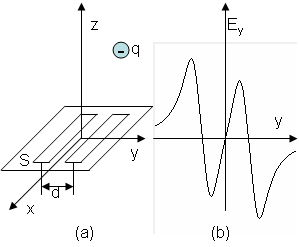
\includegraphics{2slits.png}
\caption{a) A conducting surface S is placed at plane z=0. On the surface, there are 2 slits along x axis with their centers at (0,-d/2,0) and (0,d/2,0) respectively. A negative charge q is passing at (0,y,z). b) Sketch of the lateral component of the induced electric field at the location of the charge q}
\label{fig:Double_Slit}
\end{figure}
In an approach similar to the case of one slit, define $S_1$ the area inside the slit \#1, $S_2$ the area inside the slit \#2, then $S+S_1+S_2$ is the entire plane z=0, and the integral in (\ref{eqn:Ey}) can be decomposed
\begin{eqnarray}
\int_{S+S_1+S_2} dE_y=\int_{S} dE_y+\int_{S_1} dE_y+\int_{S_2} dE_y
\label{eqn:Ey0_2}
\end{eqnarray}
again, the left side vanishes due to (\ref{eqn:Ey0}), then
\begin{eqnarray}
E_y|_{2slits}=\int_{S} dE_y=-\int_{S_1} dE_y-\int_{S_2} dE_y
\label{eqn:Ey2}
\end{eqnarray}
With (\ref{eqn:Ey1}), the integral over $S_1$ in (\ref{eqn:Ey2}) is the lateral component of induced field of slit \#1, the integral over $S_2$ in (\ref{eqn:Ey2}) is the lateral component of induced field of slit \#2, thus $E_y|_{2slits}$ is equivalent to a superposition of induced fields of each of the slits. To certain degree, such superposition of induced fields resembles those in wave theory.

For the slit centering at (0,-d/2,0), $E_y$ can be approximated with the curve of fig. \ref{fig:Single_Slit}b shifting by -d/2. Likewise, $E_y$ of the slit at (0,d/2,0) can be approximated with the curve of fig. \ref{fig:Single_Slit}b shifting by d/2. Superposition of the two slits gives rise to the sketch of $E_y$ in fig. \ref{fig:Double_Slit}b, due to the superposition, fields at certain region cancel out, thus ripples arise.

The lateral component $E_y$ of the induced field will alter the trajectory of charge q. Under the impact of $E_y$, the charge q tends to aggregate at certain area along the y axis, while escape other area. For $E_y$ of the shape as in fig. \ref{fig:Double_Slit}b, fringe like spatial distribution can arise.

As eqn. (\ref{eqn:Ey1}) and (\ref{eqn:Ey2}) show, the lateral component $E_y$ of the induced field is derived by integration over the whole surface S, with all slits on the surface excluded from the integration. Thus all slits contribute (in a subtractive way) to define the surface over which the integral is computed. Therefore $E_y$ is dependent on all slits on the surface S, which subsequently have impact on the motion of charge q, even if the charge q does not pass through some of the slits. 

In addition to define the surface of integration, slit(s) also have impact on the integrand in (\ref{eqn:Ey1}) and (\ref{eqn:Ey2}). In the above treatment of single and double slits, the induced surface charge density $\sigma$ is assumed to be the same as if the surface has no slit, this is not strictly precise, as the surface charge density (\ref{eqn:Sigma}) is derived from boundary condition (\ref{eqn:Dirichlet0}). When the surface contains slits of various configurations, the boundary condition is different from (\ref{eqn:Dirichlet0}), then the induced charge density deviates from eqn. (\ref{eqn:Sigma}), and $E_y$ varies accordingly.

The self induced field is present when the passing charge is on either side of the surface. Even after charge q passed the slit, change of the surface configuration (e.g. shut one slit) can still alter the distribution of the induced surface charge, thus affect the motion of the charge q.

The presented analysis is only dealing with one particular setup among various possible situations. In one variation, the above analysis assumes a conducting surface S. In real experiments, the surface can be dielectric, so the induced charge density differs from eqn. (\ref{eqn:Sigma}).

In another variation, the above analysis only deals with charged passing particle q, in reality, the passing particle can be molecules, which lacks free charge. However, while a non-polarized molecule (such as $H_2$) does not induce any charge on the surface, a polarized molecule (e.g. HCl) carries electric dipole, which can still induce surface charge and impact its own motion. Furthermore, one can also expect the magnetic dipole moment of a passing particle to induce some interaction with the surface.

To apply the conceptual model of self induced force in the various cases of charged particle, polarized/non-polarized molecule or conducting/dielectric surface, a thorough analysis of the lateral component $E_y$ of induced field should take those different configurations into account, so that each case can be treated in an appropriate way accordingly. This is in contrast to wave-particle duality, which takes a uniform approach, without differentiating the various scenarios.

The impact of induced charge can change the motion, thus spatial distribution of the passing particle, which is similar to the effect of wave-particle duality. Questions then arise, is the self induced force independent of the wave particle duality? 

In the case that the model of self induced force is somehow related to wave-particle duality, what is the relationship between the two models? Since the presented self induced force is deterministic, it is unlikely that the probabilistic wave-particle duality is underlying the self induced force. Then can the self induced force actually lie at the root of wave-particle duality?

If the model of self induced force is completely unrelated to the wave-particle duality, when a particle passes through the slit(s) on a surface, its motion is impacted by both the self induced force and the wave-particle duality independently. The outcome would be a combination of the two models and deviate from either pure wave-particle duality, or pure self induced force. As wave-particle duality takes a uniform approach, without differentiating charged particle, polarized molecule, non-polarized molecule, or conducting vs dielectric surface, it seems insufficient to account for all scenarios of the self induced force.

%\begin{acknowledgments}
%I am grateful to my family for their support and encouragement.
%\end{acknowledgments}

\begin{thebibliography}{0}
\label{sec:TeXbooks}
\bibitem{Juffmann} Thomas Juffmann et al, Nature Nanotechnology 7, 297-300 (2012).
\bibitem{Bach} Roger Bach et al, New J. Phys. 15 033018 (2013).
\bibitem{Jackson} J. D. Jackson, Classical Electrodynamics, 3rd ed., (Wiley, New York, 1998).
\end{thebibliography}
\end{document}
